\documentclass{article}
\usepackage[utf8]{inputenc}
\usepackage{amsmath, amsthm, amssymb, amsfonts, MnSymbol, mathtools, tikz, fancyhdr, titling, comment}
\usepackage[a5paper, top=2cm, , bottom=2cm, left=1cm, right=1cm]{geometry}
%\usepackage[a4paper, top=2cm, bottom=2cm, left=4.1cm, right=4.1cm]{geometry}

\usepackage{graphicx}
\graphicspath{{./}}

\title{Quora Insincere Questions Classification}
\author{Tristan Gregory}
\date{2018}

\pagestyle{fancy}
\fancyhf{}
\rhead{Tristan Gregory}
\lhead{Quora Insincere Questions Classification}

\begin{document}
\setlength{\parindent}{0cm}

\maketitle
\thispagestyle{empty}

\section{Discussion}
\subsection{The importance of the problem}

All corners of the internet are subject to spam and hateful users, however from some websties users will expect greater levels of sanctity. Question and answer sites, especially those as multilingual and comprehensive as Quora, are held to high standards by users because it is a platform primarily for learning and sharing. Insincere questions could undermine the platforms' aims by misleading users and discouraging open discourse. Not to mention such problems if left unadressed could lead to a very cluttered website, costing Quora money and costing users their valuable time.\\

Quora is a remarkable platform used by many millions so the problem happens on a large scale and promises to continue long into the future. That is why this is an extremely important problem that cannot be overlooked.

\subsection{How machine learning might help here}

Since this happens on such a large scale, we cannot rely solely on the users for content moderation. It is likely that the majority of users don't care enough to report/ downvote insincere questions so most will slip through the net.\\

Potentially we could use a machine learning model to supplement this in a small way by only flagging questions that the model is very confident are insincere. The upside of this is a low instance of false positives, and the downside is a high instance of false negatives. This is good because removing questions that appear insincere that are in fact completely genuine would be inconsistent with the aims of the platform, and genuine users would be left with no answers to their questions. So machine learning should be used, but some of the content moderation should still fall down to the users and Quora employees.

\subsection{Which machine learning technique is most useful and why}

This is a binary text classification problem. Sentiment analysis must be performed on each question using natural language processing. I have access to four pretrained word embeddings including Word2Vec, Glove, Paragram and fastText. First though, I tried training the word embeddings myself to see what baseline accuracy I could achieve. The idea after that was to run the pretrained word embeddings through a multilayer neural network to train the model to most accurately identify insincere questions.\\

I believe this is the typical approach to such a problem. Sometimes this is the best approach - especially when using the wrong learning algorithm could mean time and money down the drain. Perhaps a different, novel ML solution exploiting a particular characteristic of the Quora question data set, or of the syntax of a question, could score higher but it may lack scalability because it might not be valid for the many other languages Quora is available in. For example, if we notice that in English taking only the last two-thirds of every question extracts more relevant information/ leads to a higher score, then the same may not apply to Italian.\\

\textit{As a side note, I'm sure there are novel ML solutions that can be generalised unlike the very simple one I just mentioned, however the effort/cost may outweigh the return. For example, maybe we could wrap a highly simplified/optimised logistic regressor model in a layer of a larger logistic regressor with an input vector made up of variables such as the dimension of the embeddings, the maximum number of words and the maximum length of each question. However this is essential a nested neural network and likely to have a very high time complexity and hence a costly approach.}\\

I actually tried building a Naive Bayes model for faster runtime however it was hitting scores of around 0.5 so I did not take this model any further. I have included this ipython notebook too for sake of interest. It would work well as a super fast model that can give immediate results reasonably accurately, however as a full solution it does not cut it. Similarly I saw no significant increase in score when blending multiple pretrained embeddings so for simplicity I did not include this in the final kernel.

\section{Implementation}
\subsection{The model and its in-sample, out-of-sample (leaderboard) performance}

The model is fully explained in the notebook. The highest private score from the notebook was 0.681 which was achieved at a threshold of 0.43. My highest public score was 0.677 as you can see below.

\textbf{Note: Due to post-competition dataset changes, my original kernal became invalid and so I had to rerun the notebook. My new private score was 0.666 and my new public score was 0.659.}

\begin{center}
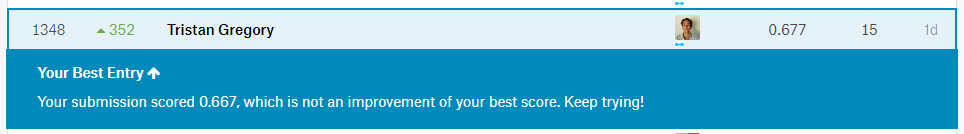
\includegraphics[width=12.8cm]{leaderboard.png}
\end{center}

The only part of the model I did not explain in the notebook was the particular choice of layering, so I will do this here instead. For convenience, I have included the model summary from the notebook below.

\begin{center}
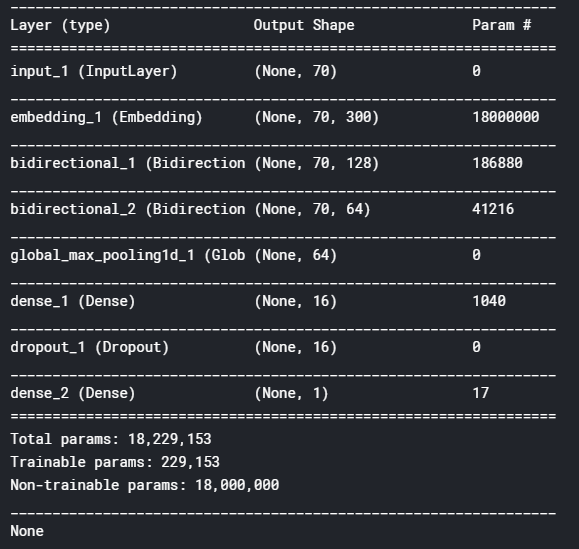
\includegraphics[width=8cm]{summary.png}
\end{center}

The embedding as we can see is taking 70 word vector embeddings, each with dimension 300. All of these are non-trainable parameters (making them trainable would massively increase time complexity). Then we have two bidirectional LSTM layers one after another training any words not covered by the Glove embedding, and reducing their dimension down to 128, and then 64. Then the GlobalMaxPool layer produces a maximum vector for each message with an output dimension of 64. The dense layer is a fully connected layer that further reduces the dimension of the vector for each message to 16. Then I have included a dropout layer which randomly removes one of the input neurons with an aim to reduce overfitting. Finally we have a dense layer condensing the output into a single variable between 0 and 1. This output neuron represents how insincere the model thinks a particular question is.

\section{Remarks}
\subsection{Advice on how to implement this model in production to make the site safe for everyone}

In production, the model may not perform as well because the data may not be quite so clean (e.g. large quantities of bot generated questions etc). This is to be expected and further measures can be taken on a case by case basis to address any inconsistencies that arise. As a general rule of thumb, we will favour false negatives over false positives (as explained earlier on) by setting the threshold slightly higher in production than on Kaggle. The model may have to be trained on a regular basis because the distribution of questions may change depending on political events etc, and this may affect the accuracy of the model. Providing this training data on a regular basis may require a significant amount of human resources so the intervals over which retraining takes place should be carefully decided.\\

Also, if we wish to see how it's training the word vectors, we could use TSNE to visualise the word vectors as a 2D diagram. Understanding this could help debug, reduce overfitting, explain behaviours, and inform layer tweaks.\\

I can provide no further advice however I suggest adding an attention layer for a slightly improved model. That said, the model has performed quite well without the attention layer, so if running time is a big factor then we don't need to add anything. However if running time isn't really an issue then a well configured attention layer may make a good addition to this model.
\end{document}